  \mysection{The Mystic}{trope-mystic}

  \flavor{Creedsmen roll out across the dying dawn - Sacred Israel holy mountain Zion - Sun beams down on to the sandsea reigns - Caravan migrates through deep sandscape - Lungsmen unearth the creed of Hasheeshian - Procession of the weed-priests to cross the sands - Desert legion smoke-covenant is complete - Herb bales re-tied on to backs of beasts - Arise arise arise - The Son of the God of Israel - Jordan river flows on evermore - Bathe in glow of sunlight's beating rays - They feel the serpent's standard rule our day \Tilde Sleep, "Dopesmoker"}

  \begin{center}
  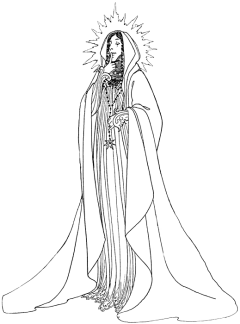
\includegraphics[scale=.5]{Mystic}
  \end{center}

  \cbreak


  \mysubsection{The Basics}{mystic-basics}

  \myhighlight{Squishy}{mystic-flesh}

  Mystics have a d4 \FLESH

  \myhighlight{Contemplative}{mystic-contemplative}

  Mystics add their \LVL to any \RO or \RB attempt they're trying that includes their \FOC


  \mysubsection{Creation}{mystic-creation}


  \callout{
    \mynumlist {
      \item Move any of your core Skills \DCUP
      \item Move any of your core Saves \DCUP
      \item Pick \mybold{three} \mylink{Virtues}{mystic-virtues} from the list below.  You can only pick each Virtue once.
      \item Pick \mybold{one} \mylink{Complication}{mystic-complications} from the list below (or make up your own with the Arbiter!)
      \item Write down your Starting Gear
    }
  }



    \mytable{X}{
      \thead{\mysubsection{Virtues}{mystic-virtues}} \\
    }{
      \mylink{Aura}{mystic-virtue-aura} \\
      \mylink{Charms}{mystic-virtue-charms}  \\
      \mylink{Cunning}{mystic-virtue-cunning} \\
      \mylink{The Crux of Mojo}{mystic-virtue-mojo} \\
      \mylink{The Crux of Faith}{mystic-virtue-faith} \\
      \mylink{The Gift of Grace}{mystic-virtue-grace} \\
      \mylink{Initiate}{mystic-virtue-initiate} \\
      \mylink{Intangibles}{mystic-virtue-intangibles} \\
      \mylink{Liturgies}{mystic-virtue-liturgies} \\
      \mylink{Necromancy}{mystic-virtue-necromancy} \\
    }


    \myhighlight{Aura}{mystic-virtue-aura}

    If you possess the \mylink{Crux of Mojo}{mystic-virtue-mojo} Virtue, you may use your Mojo as both armor and weapon. 

    If you are struck in Combat, you may roll your Mojo \UD and treat the result as if you were wearing Armor.

    You may additionally shape your Mojo into a Brawl weapon of your choice.  The weapon uses your \FOC for Fight and deals your Mojo \UD in damage. 

    Wearing armor, a shield, or a helmet; or using a weapon interferes with your Aura.  You can't use your Aura if you're so armed or attired.

    Describe to the Arbiter what this mystical armor and weapon look like.

    \myhighlight{Charms}{mystic-virtue-charms}

    You may cast \mylink{Charms}{arcana-charms} and cantrips at will

    \myhighlight{Cunning}{mystic-virtue-cunning}

    Your fate is also now intertwined with the waxing and waning of the 5 moons and Tartarus.  You gain a \mylink{Familiar}{occultism-bind-familiar} with a strength of 5, and 2 points of Cunning.

    Cunning is used during a \mylink{Vacation}{civilization-vacation} to perform the \mylink{Marvel of Occultism}{marvels-occultism}, and be used to help Spriggans practice \mylink{Sword Magic}{spriggan-sword-magic}.  Cunning is bound to the Wheel.

    \mybold{The Wheel}

    Your Cunning moves counterclockwise through a Wheel of eight points - it ascends from the Void to Sickle, Quotidian, and Gibbous to Crown, then descends through Gibbous, Quotidian, and Sickle to return to the Void.  The phases of the Wheel will grant you extra Cunning in your occult practices (see the section on \mylink{Occultism}{marvels-occultism}.
  
    When you first take this Virtue, roll a d8 to see where your Mojo begins:

    \mytable{X X}{}
    {
      1 & Void \\
      2 & Waning Sickle \\
      3 & Waning Quotidian \\
      4 & Waning Gibbous \\
      5 & Waxing Sickle \\
      6 & Waxing Quotidian \\
      7 & Waxing Gibbous \\
      8 & Crown
    }

    Every Session, move your Mojo one step counter-clockwise along the wheel:

    \begin{center}
  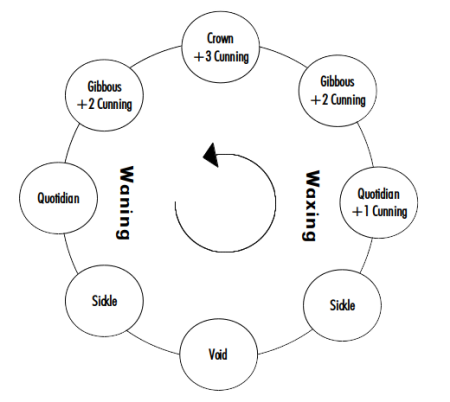
\includegraphics[scale=.5]{mojo_circle}
  \end{center}



    \myhighlight{The Crux of Mojo}{mystic-virtue-mojo}

    \flavor{True magic is not written. It is passed down, mother to daughter, since the very beginning.  It is richly colored, deeply echoing, singing in the rivers and whispering through the leaves.  The Philosopher seeks it in the Void or inside some book or rattling around at the edges of madness, but that is false magic, waiting to betray.  True magic is the pulling of a baby from the womb, knitting bones and purging poisons, reading the entrails and speaking with the crickets and seeing the patterns in the smokes. This is not some power that is beyond mortal reckoning, but a power that is here for anyone - from king to mudlark - to harness for weal or woe. The Crux of Mojo allows you to tap into the wellspring of magic to protect yourself, harm your enemies, and command the dead.}

  Gain 1 d8 Mojo \UD You can use your Mojo \UD to power your \mylink{Aura}{mystic-virtue-aura} and to practice \mylink{Necromancy}{arcana-necromancy}. 

  \begin{center}
  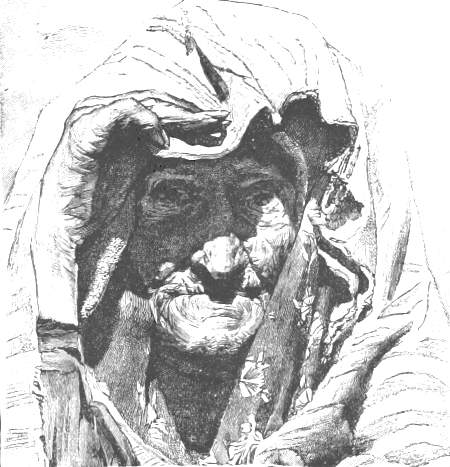
\includegraphics[scale=.5]{Mystic_1}
  \end{center}


    \myhighlight{The Crux of Faith}{mystic-virtue-faith}

    \flavor{And it has been said of old that all things that have been were wrought by the small gods, excepting only \TheAuthority, the Authority, the God of Having Done, who made the gods, and hath thereafter rested.  And none may pray to \TheAuthority but only to the gods whom he hath made. \Tilde Lord Dunsany}

    It is forbidden to worship \TheAuthority directly; instead, you whisper your prayers and invocations to the Small Gods, the Gods of Doing.  Your Faith (measured as d4 \UD) in your Small God allows you to invoke the Liturgies of the Authority they sit beneath.

    You gain 2 d4 Faith \POOL and your \MAX Faith is 4. You can use Faith to perform \mylink{Miracles}{marvels-miracle-working}, and to perform the \mylink{Liturgies}{mystic-virtue-liturgies} of one of the Small Gods.

    Unlike Grace, Faith does not come back when you rest.  You can gain or regain Faith up to your \MAX by actively, aggressively pursing your Small God's influence on Acheron.  You gain Faith \UD completely at the Arbiter's discretion.  Some examples of things that might gain you Faith: slaughtering the priest of a rival cult; converting a crowd of listeners; invoking the name of your Small God and succeeding; eating hallucinogenic mushrooms and tripping balls while your Small God copulates with you, proclaiming your destiny, etc.

    It's possible to lose Faith through your actions, as well.  When you do something your Small God doesn't approve of or witnesses something which would shake your belief, you lose Faith Dice: a commune of the converted found diseased, deformed, and starved; a call for help which goes unanswered; a nocturnal visit by a creeping hulking thing which whispers terrible secrets of the endless sky into the your ear heedless to the invocation of your God.

    If your Faith \POOL is every exhausted, you must immediately roll a d4 - on a Failure (a 1 or a 2) you suffer a \mylink{Crisis of Faith}{table-crisis-of-faith}; otherwise, gain +1 Faith \UD
  
   

    \myhighlight{The Gift of Grace}{mystic-virtue-grace}

    \flavor{\myital{In principio erat Verbum} \\~ \Tilde John 1:1}


    The Holy Word of \TheAuthority echoes and reverberates along the branches of Ygg.  The act of trying to understand the Word bestows Grace of \TheAuthority on you

    Gain a d4 Grace \UD.  Grace Dice are \POOL, meaning if you roll a Failure (a 1 or a 2) you lose the die until you rest.  You can restore up to 2 Grace \POOL whenever you Bivouac. 

    You can never use Grace to perform something that requires Faith, but it will allow you to perform the \mylink{Seven Sacraments}{arcana-seven-sacraments}.
 
    \newpage

    \myhighlight{Initiate}{mystic-virtue-initiate}

    You are no stranger to the trials and travails of life; you have accumulated some gear on your journeys.  You can pick \mybold{three} of the following:
    \dashedbox{
    \mybullet {
      \item a Fast weapon of your choice;
      \item a Hard weapon of your choice;
      \item a Magical athame (treat as a normal dagger that can strike creatures only affected by magic);
      \item a suit of Light armor;
      \item a suit of Medium armor;
      \item 5 picks from the \mylink{Adventuring Gear}{gear-adventuring} table;
      \item a pouch of 3 gems (roll on the \mylink{Gems table}{appendixb-random-treasure} in Appendix B);
      \item d4 \UD of 3 different Narcotics, or d10 \UD of one;
      \item a \mylink{Mule}{gear-transport};
      \item 3 rumors from the Arbiter about your first adventure.  These rumors can be opaque but they must be true.
    }}


    \myhighlight{Intangibles}{mystic-virtue-intangibles}

    You may move two different Intangible Stats of your choice \DCUP.  Describe to the Arbiter why these Intangible Stats are better than average.

    \myhighlight{Liturgies}{mystic-virtue-liturgies}

    Requires the Crux of Faith.  Choose an \mylink{Authority}{mystics-authorities} and a Small God who sits beneath it (this can be a Small God that's listed, or a Small God of your choosing).  You learn the \mylink{Liturgy of the Novitiates}{mystics-authorities} of that Small God, and can perform it using the Crux of Faith.  You also gain a Holy Symbol with 1 Faith \POOL "inside" of it

    \myhighlight{Necromancy}{mystic-virtue-necromancy}

    Using your Mojo, you can question and command the dead, and use your black magics to heal.  More information can be found in the \mylink{Arcana: Necromancy}{arcana-necromancy} section


  \mytable{X}{
    \thead{\mysubsection{Complications}{mystic-complications}} \\
  }{
    Animal Lover \\
    Burn the Witch! \\
    Cat's Eyes \\
    Heretic \\
    Imma Smoke It \\
    My Name is Earl \\
    Otherworldly \\
    Transubstantiation \\
    The Unseelie \\
    Vow of Poverty 
  }

  \myhighlight{Animal Lover}{mystic-animal-lover}

  You love all kinds of animals; you refuse to ride beasts of burden (including being pulled in a cart by them), eat meat, or suffer the mistreatment of an animal (does not apply to animals that are actively trying to kill you).

  \myhighlight{Burn the Witch!}{mystic-complication-witch}
  
  Any time you stay in a Tiny Civilization, you run the risk of being accused of witchcraft.  If you stay in a Tiny thorp, dorf, etc. roll 2d6 - on a 2 (snake-eyes) you're accosted for poisoning the well water / getting the farmer's daughter pregnant (your gender is irrelevant) / making the chickens sick, etc. If you roll a 12 (boxcars), you'll be called on to do something important - deliver a baby, heal someone's fever, etc.

  \myhighlight{Cat's Eyes}{mystic-cats-eyes}

  Through some mishap, you have the eyes of a cat.  They unfortunately don't allow you to see very well in the dark (treat as if you were holding a candle, probably enough to read by but not much else).  They glow in the dark, however, making it difficult (though creepy) to sneak up on the unwary

  \myhighlight{Heretic}{mystic-complication-heretic}

  Name a Small God.  This God is heretical to your belief; its followers must be slain, its temples desecrated, and its name forgotten

  \myhighlight{Imma Smoke It}{mystic-imma-smoke-it}

  You're constantly looking for new and better ways to transcend the mortal plane and see into the heart of the universe i.e. to get high.  If there's a weird mushroom, you're going to try it.  Some kind of slime, put it in your pipe and see what happens.  I hope you've decided to bump your Toxins Save.

  \myhighlight{My Name is Earl}{mystic-name-is-earl}

  You have set out on the path of the Mystic thanks to the help and sacrifice of another.  You can never repay this debt, so you must pay forward kindness whenever possible.  Tell the Arbiter what this debt is, and who you owe it to.

  \myhighlight{Otherworldly}{mystic-otherworldly}

  You are eerie, uncanny, and unreal.  You don't cast a reflection, and your footprints appear backwards.  Common folk want nothing to do with you; more powerful persons you meet hold you at arm's length.

  \myhighlight{Transubstantiation}{mystic-transubstantiation}

  Requires Cunning or the Crux of Faith.  Your Occultism and Miracles are fueled by your own flesh and blood - not a lot, anywhere between a few drops and a goblet-full; a small slice off a limb to a fingertip's worth.  The effects of using your own flesh and blood in this way can have ... interesting effects ... at the complete discretion of the Arbiter.

  \myhighlight{The Unseelie}{mystic-unseelie}

  The Unseelie are Unhallowed, anathema in the eyes of the Authority.  The Unseelie deserve your contempt at best, to be burned at the stake at worst.

  Alternately, the Unseelie are cursed and alone.  The deserve your pity and understanding, and to be protected from the infantile fears and hatreds of Mortals.

  \myhighlight{Vow of Poverty}{mystic-vow-of-poverty}

  You have taken a vow of poverty.  You will never possess more money than you need to live a basic existence; you live as humbly as you possibly can.  You still insist on your full share of treasure, but you will donate it or give it away.  The donation must be anonymous, and you cannot gain Faith in this way (though you can gain Glory if you spend this money during a \mylink{Vacation}{civilization-vacation}).

  \cbreak

  \mysubsection{Starting Gear}{mystic-starting-gear}

  \mybullet {
    \item a quarterstaff and dagger; 
    \item 2 iron pieces;
    \item a pipe and d4 \UD of tobacco;
    \item 3 picks OR 5 rolls on the \mylink{Random Items}{appendixb-random-items} table in Appendix B;
  } 

  

  \mysubsection{Examples}{mystic-examples}

  \myhighlight{The Wandering Monk}{mystic-example-wandering-monk}

  \example{Bushcraft, Crux of Mojo, Aura, Seven Sacraments, Animal Lover}

  \myhighlight{The Shaman}{mystic-example-shaman}

  \example{Lore, Crux of Mojo, Aura, Necromancy, Otherworldly}

  \myhighlight{The Witch}{mystic-example-witch}

  \example{Lore, Crux of Mojo, Charms, Cunning, Burn the Witch!}

  \myhighlight{The Pilgrim}{mystic-example-pilgrim}

  \example{Travel, Crux of Faith, Seven Sacraments, Liturgies, The Unseelie}


